%% Individual Progress Report.tex
%% ZJUI Senior Design Individual Report

\documentclass{senior-design-individual}
\graphicspath{{Figures/}}
%%% Report information %%%%%%%%%%%%%%%%%%%%%%%%%%%%%%%%%%%%%%%%%%
%TODO: Fill project info here
\semester{Spring 2025}
\reporttitle{Human-Robot Interaction for Object Grasping with Virtual Reality and Robotic Arms}
\projectnumber{26}
\supervisor{Gaoang Wang \& Liangjing Yang}
\ta{Tielong Cai \& Tianci Tang}
\reportdate{April 17, 2025}

%TODO: Fill personal info here
\authorname{Ziming Yan}
\studentid{zimingy3}
\grade{2021}
\major{Electrical Engineering}
%%%%%%%%%%%%%%%%%%%%%%%%%%%%%%%%%%%%%%%%%%%%%%%%%%%%%%%%%%%%%%%%%
\addbibresource{references.bib}  % bib database
\begin{document}
% Coverpage
\begin{titlepage}
    \newgeometry{left=1cm, right=1cm, top=1in, bottom=1in}
    \begin{center}
        ~~\\ % to make the vspace effective
        \vspace{1.5cm}
        {\fontsize{16}{24}\selectfont Zhejiang University-University of Illinois Urbana-Champaign Institute}\\
        \vspace{1.88cm}
        {\fontsize{28}{42}\selectfont Individual Progress Report}\\
        \vspace{1.6cm}
        \begin{minipage}{15.92cm}
            \centering
            \fontsize{26}{26}\selectfont
            \MakeUppercase{\bf \RPTTITLE}
        \end{minipage}\\[2cm]
        % {\fontsize{14}{21}\selectfont By}\\[1.5em]
        \begin{table}[h]
            \centering
            \fontsize{14}{12}\selectfont
            \renewcommand{\arraystretch}{1.5}
            \begin{tabular}{cc}
                NAME:&Ziming Yan\\
                UIN:&zimingy3\\
            \end{tabular}
        \end{table}
        \vfill
        {\fontsize{12}{\baselineskip}\selectfont Individual Report for Senior Design, Spring 2024\\
            Major: \MAJOR \\
            % Grade: \GRADE \\
            Supervisor: \FACULTYNAME \\
            TA:~ \TANAME\\
            \vfill}
        {\fontsize{12}{18}\selectfont\RPTDATE\\
            Project No. \PROJNBR}
    \end{center}
    \vspace{2cm}
    ~
    \restoregeometry
\end{titlepage}
\tableofcontents
\mainmatter
%%% Body %%%%%%%%%%%%%%%%%%%%%%%%%%%%%%%%%%%%%%%%%%%%%%%%%%%%%%%%
% TODO: Main body starts here
\chapter{Introduction}
\section{Project Overview}
Current robotic systems lack intuitive and seamless human-robot interaction for
object manipulation. Traditional teleoperation methods often require complex con-
trollers, making it difficult for users to interact naturally. With advancements in Virtual
Reality (VR) and robotic systems, it is possible to develop an intuitive interface where
users can manipulate objects in a virtual space, and a robotic arm replicates these ac-
tions in real-time. This project aims to bridge the gap between human intention and
robotic execution by integrating VR with robotic grasping, enabling precise and effi-
cient remote object manipulation. Such design opens up to a wide potential market
catering to various customer needs, such as remote working with precise control of
streamline, dining requests of the Parkinson's, etc.
 
To be specific, our solution addresses the problem by the following workflow:
First, we create a digital twin of the target objects alongside the robotic arm in Unity
environment. Then we connect it with the Meta Quest VR App and render the scene,
which is updated in real-time. During runtime, the Quest reads in the user's hand
trajectory so that it will be able to recognize which target object to grasp. It constantly
returns this information together with the hand trajectory to the control module on
PC. The control module calculates a set of recalibrated waypoints and sends to ROS,
which orders the robotic arm to approach the object in a way that simulates the user’
s grasping trajectory.
\begin{figure}[h]
    \centering
    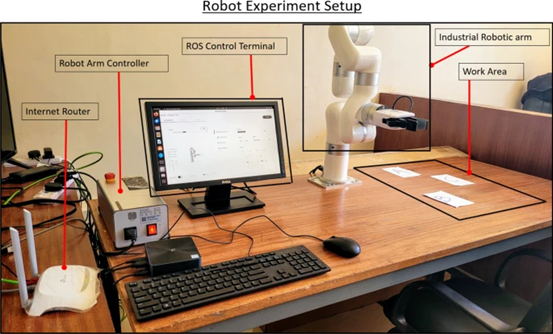
\includegraphics[width=0.8\linewidth]{Robot Experiment Setup.png}
    \caption{Design Concept}
\end{figure}
\section{Responsibilities and Role}
As the only electrical engineering student in the team, I have a certain knowledge base of embedded chip control development, motor control and robotic arm operation. In addition, I have knowledge of mechanical structure and 3D modeling in my spare time as well as in my research projects. Therefore, I was also responsible for related tasks in the project. Specifically the following aspects:
\begin{enumerate}
    \item Design the overall task division of the project and draw a Block Diagram
    \item Record the progress of the experiment and test data in the lab notebook.
    \item Configure the STM32 programming environment and debug the STM32F407 development board.
    \item Control the development board to realize the communication with the stepper motor driver board, and then control the stepper motor.
    \item Modeling and optimizing the mechanical gripper with mechanical students to control the UR3 arm.
\end{enumerate}
\chapter{Individual Design Work}
\section{Design and Draw the Block Diagram}
The most important task of the project, before starting the division of labor, 
is the structural distribution, i.e., dividing the functions to be implemented 
into specific modules and assigning them to each person according to his 
characteristics, specialties and strengths. I initially divided the project 
into four subsystems: Mixed Reality (MR), Digital Twins, Control System, and Robot 
Arm, but after talking with my mentor Yang Liangjing in the group meeting and 
discussing among the members, I decided to add an auxiliary positioning system 
to improve the accuracy of the clamping, which is assisted by an external 
positioning camera. 
 
In addition, due to the limitation of MR devices of campus (It has been used in other projects before the construction of our project), we changed our original design with MR to virtrual reality (VR), and use the hand tracking technology to record the track of hands. With The use of handles would increase the accuracy of route recording, but at the same time increase the difficulty of writing the program. After going through the process of communicating with Jiayu Zhou, who is responsible for writing the program, he agreed to this change. The final Block Diagram is shown below:
\begin{figure}[h]
    \centering
    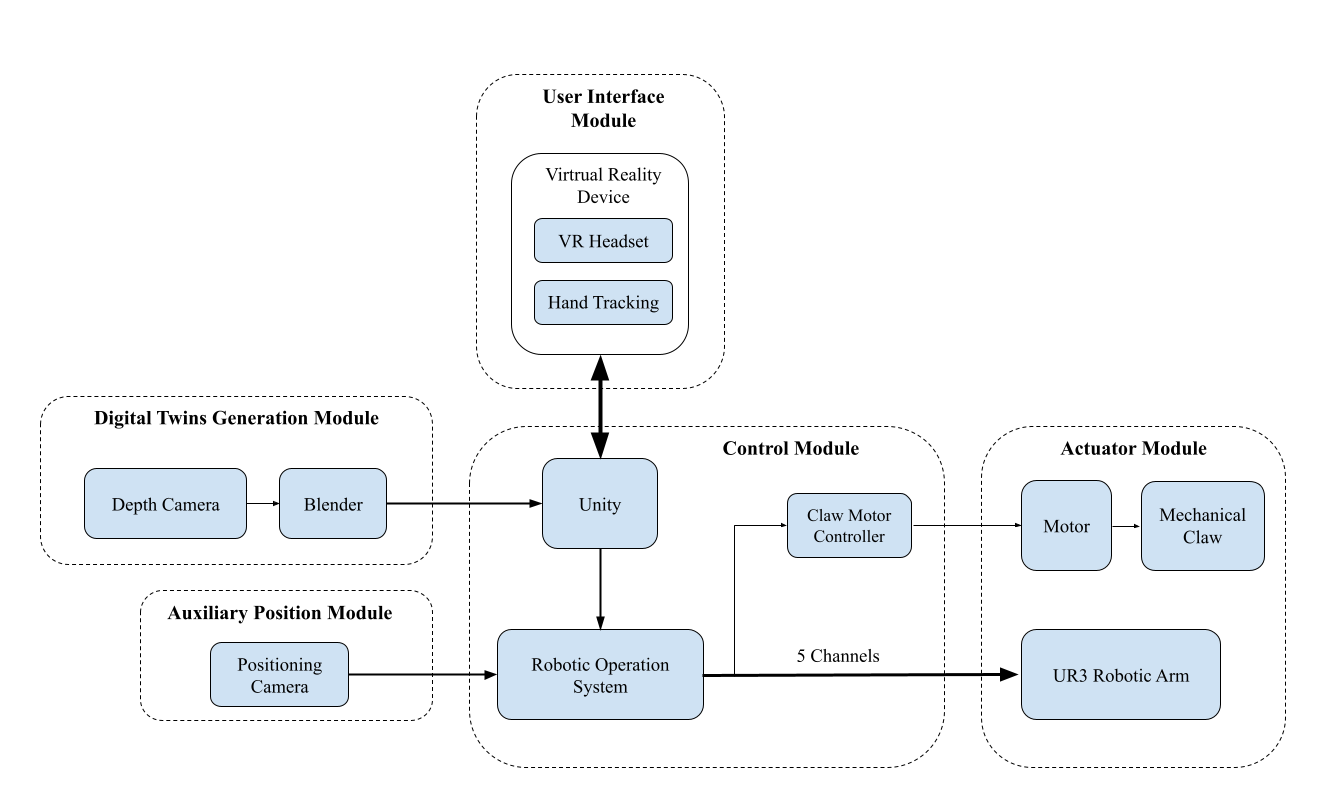
\includegraphics[width=0.8\linewidth]{Block Diagram.png}
    \caption{Block Diagram}
\end{figure}
 
\section{Control Module}
    \begin{itemize}
        \item \textbf{Unity Integration:} The Unity will receive the data flow from VR hand tracking and transmit it to the ROS to compute the route of robot arm. In addition, it uses the 3D data from depth camera to reconstruct the environment.
        \item \textbf{ROS (Robotic Operating System) Communication:} According to the position information of hands from Unity, ROS could computed the track into parameters of motors to control 5 robot arm joints and pass signal to STM32 motor control board.
        \item \textbf{Motor Controller:} Use STM32 control board to control motor speed, angle and other information with closed loop control.
    \end{itemize}
 
As for me, I was responsible for implementing and programming motor controller firstly. At first, I wanted to use STM32F104 development board and SG90 rudder to drive the claw and the Jingxing Hu also used rudder parameters to design to 3D model. Through refering to files and websites, I learned how to construct the STM32F103 board compiling environment Keil-MDK \cite{csdn_daniaoxp_2025} and successfully burned some simple programs as tests.
 
After that, I generate output PWM signal via SWD interface of STM32F103 board to control the angle of SG90 servo. 
\begin{figure}[h]
    \centering
    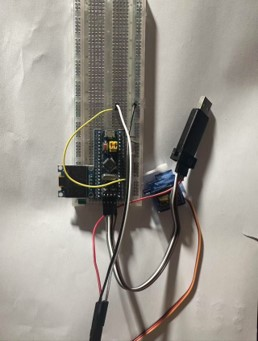
\includegraphics[width=0.6\linewidth]{STM32F103.png}
    \caption{Servo Motor Controlled by STM32F103}
\end{figure}
 
Though, the servo was able to drive the claw, it cannot achieve the close loop control. The servo motor was too simple with PWM control, and the torch it applied was also small which could not match our design. Therefore, I wanted to change it to stepper motor, and use STMF407 board to realize the close loop control. After discussion with mentors, they approved my suggestion.
The STM32F407 chip has better M4 core and can operate with higher frequency signal compared with F103, which means its control signal would be more accurate. There needs to explain that the 42 stepper motor should be controlled with 4 lines, 2 poles. So, it always needs drive board to control. As for my project, I decided to use Emm42\_V 5.0 board to control. The reason is that this board can offer close loop control with same physical demension with motor, I can attached to the back of motor to save space. The following figure shows my design of new control system of stepper motor.
\begin{figure}[h]
    \centering
    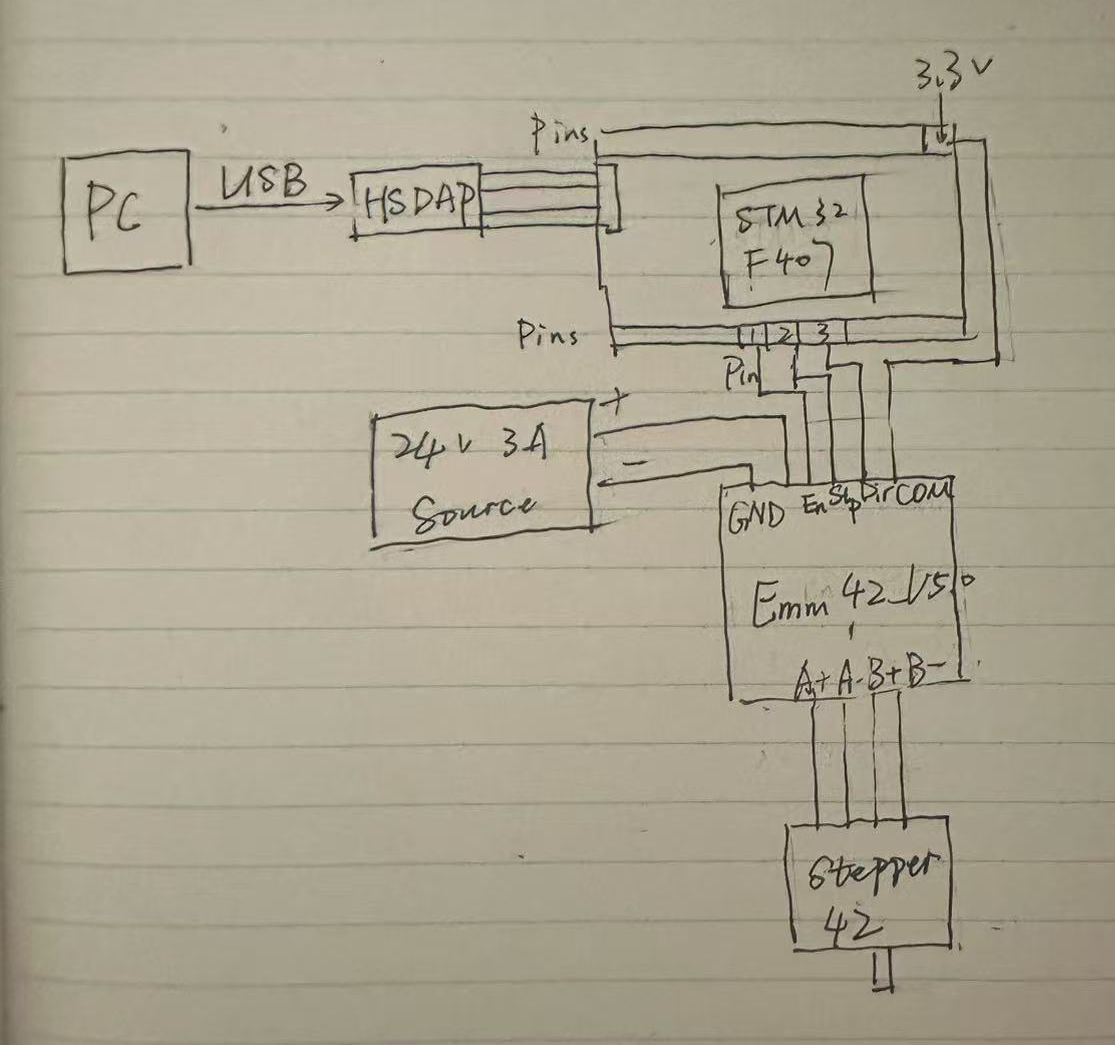
\includegraphics[width=0.8\linewidth]{Motor Controller.png}
    \caption{Motor Controller Design Graph}
\end{figure}
\section{Design Verification Approach}
While writing the design document, I wrote the Tolerance Analysis. Through learning essays and thinking verification test, I got the limitation of UR3 robot arm and motor, including the approaches to test verification.
\subsection{UR3 Robot Arm}
There are limitations to robotic UR3, ensuring that it can accurately move 
following the computed route. Motivation speed is one of the most important 
factors. As mentioned in the instruction document, the general speed tolerance 
is -150mm/s. This means that if the user configures a 250mm/s speed limit, then 
the maximum operational speed will be 250-150=100mm/s. Safety tolerances 
prevent safety violations while allowing for fluctuations in program behavior. 
For example, when handling a heavy payload, there may be situations where the 
Robot Arm needs to briefly operate above the normal maximum operational speed to 
follow a programmed trajectory \cite{ur3-manual}. An example of such a situation is shown in 
figure. 
\begin{figure}[H]
    \centering
    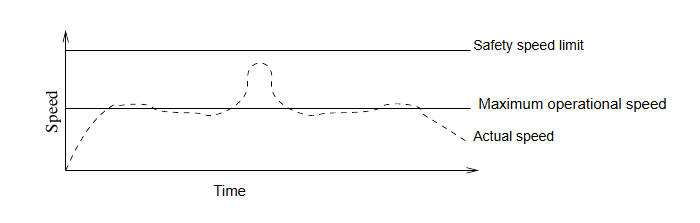
\includegraphics[width=0.8\linewidth]{UR3 Tolerance.png}
    \caption{Safety Tolerance Example}
\end{figure}
\subsection{Torch of Grasping}
The precision of grasping, especially whether the claw could successfully hold 
on to the items, mostly relies on the force of the claw applied. In other words, 
it depends on the torch range that the motor could supply. To verify the 
feasibility of our design, we want to use FEA ( Finite Element Analysis) 
software, like ANSYS, COMSOL, or Abaqus.
 
For example, the object material is plastic and can obtain 60 MPa 
maximum stress before damage. The friction coefficient ($\mu$) is 0.3. After 
simulation, we find we need to apply 15N force on the object, the contact area 
is $3mm^2$, according to the formula: 
\begin{equation*}
    Pressure(P)=\frac{Force(F)}{Area(S)}=\frac{15}{3} \cdot 10^{-6}=5MPa<60MPa 
\end{equation*}

We could ensure claw will not break the object if grasped successfully. Therefore, we could compute the corresponding Torch(T) with formula: 
\begin{equation*}
    Torch(T)=Length(L) \times Force(F)
\end{equation*}
\section{Digital Twins Generation Module:}
I learned related knowledge to help the digital twin development of Yuchen Yang. The environment is scanned by a depth camera to get a 3D point cloud file. The depth data can be reconstructed into a 3D mesh by the SDK or plug-ins in Unity3D \cite{unity_camera_reference_2024}, and reconstructed into a virtual environment consistent with reality through Unity3D rendering \cite{unity_mesh_renderer_6000}.
\section{Record Research Notebook}
As I mentioned in the introduction, I was responsible for the recording of progress in the research notebook. For example, when Jingxing needs parameters of UR3 robot arm and servo motor at the beginning of 3D modle development, I recorded all the parameters needed in the notebook. In addition, I recorded the discussion and ideas for the future research.
\begin{figure}[h]
    \centering
    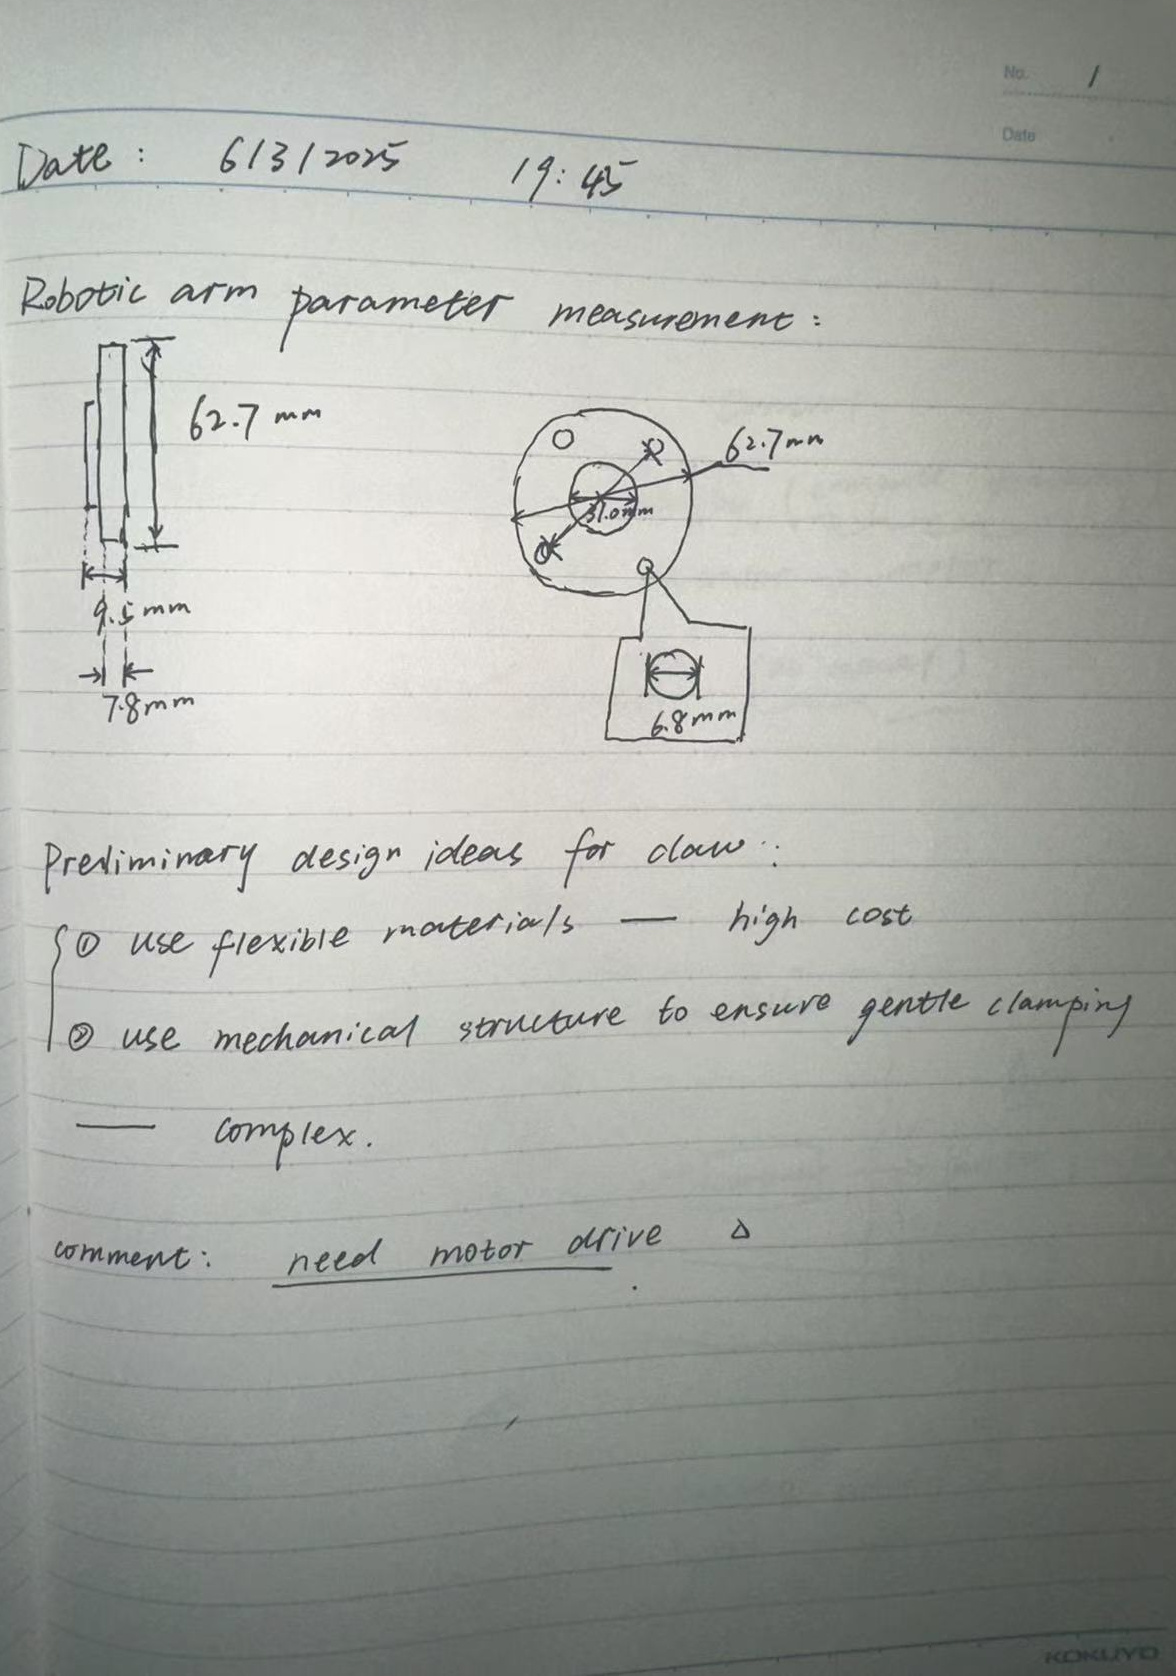
\includegraphics[width=0.6\linewidth]{notebook.png}
    \caption{Notebook}
\end{figure}
\chapter{Conclusion}
\section{Self-assessment}
Up till now, I have finished the STM32F407 board initialization successfully. Actually, my assignment progress is slightly behind of my schedule. I think the reason for the formation of this situation is that the preliminary route does not match the expected results, such as the preliminary F103 development board and servo combination can not meet the project requirements after a series of understanding before deciding to change to 42 stepper motor and F407 this trial and error time cost is higher. In addition, in the STM32F407 chip debugging to modify the loopholes and knowledge of stepper motor control knowledge also spent more time.
 
Although the progress is not the fastest, I think I played many irreplaceable roles in the team, such as the contribution of thinking during the discussion process, the presenter-sharer in the group meeting discussion, slides production, and report writing, which cannot be shown in the form of words and pictures. Overall, I think we will be able to complete our Senior Design successfully.
\section{Plans for remaining work}
\begin{table}[h]
    \centering
    \renewcommand{\arraystretch}{1.5}
    \begin{tabular}{|l|l|}
        \hline
        \textbf{Duration} & \textbf{Milestone} \\
        \hline
        1 Week & Compile and burn STM32 code and debug by linking to stepper motor \\
        \hline
        1 Week & Connect the claw control signal from ROS to STM32 \\
        \hline
        1 Week&Realize the closed-loop control of the motor\\
        \hline
        1 Week & Test the grasping and finish the Final Report \\
        \hline
    \end{tabular}
\end{table}
%%%References%%%%%%%%%%%%%%%%%%%%%%%%%%%%%%%%%%%%%%%%%%%%%%%%%%%%
\clearpage
\renewcommand*{\UrlFont}{\rmfamily}
\printbibliography[title={References},heading=bibintoc]
\clearpage
%%%%%%%%%%%%%%%%%%%%%%%%%%%%%%%%%%%%%%%%%%%%%%%%%%%%%%%%%%%%%%%%%
\end{document}